\chapter{Holding positions}

	\section{Introduction}
	\paragraph{} Because traffic density will be medium or heavy, holding bays will be designed. Hence, runway-holding positions will be established:
	on the taxiways, at the intersection of a taxiway and a runway and at an intersection of a runway with another runway when the former runway is part of a standard taxi-route.
	
	A runway-holding position will be established on a taxiway if the location or alignment of the taxiway is such that a taxiing aircraft or vehicle can infringe an obstacle limitation surface or interfere with the operation of radio navigation aids.
	
	All the distances declared on this section will be used on the CAD model for defining each section of the airport concerning to these measures.
	
	\section{Minimum distance from the runway centre line to a holding bay, runway-holding position or road-holding position}
	
	\begin{figure}[H]
		\centering
		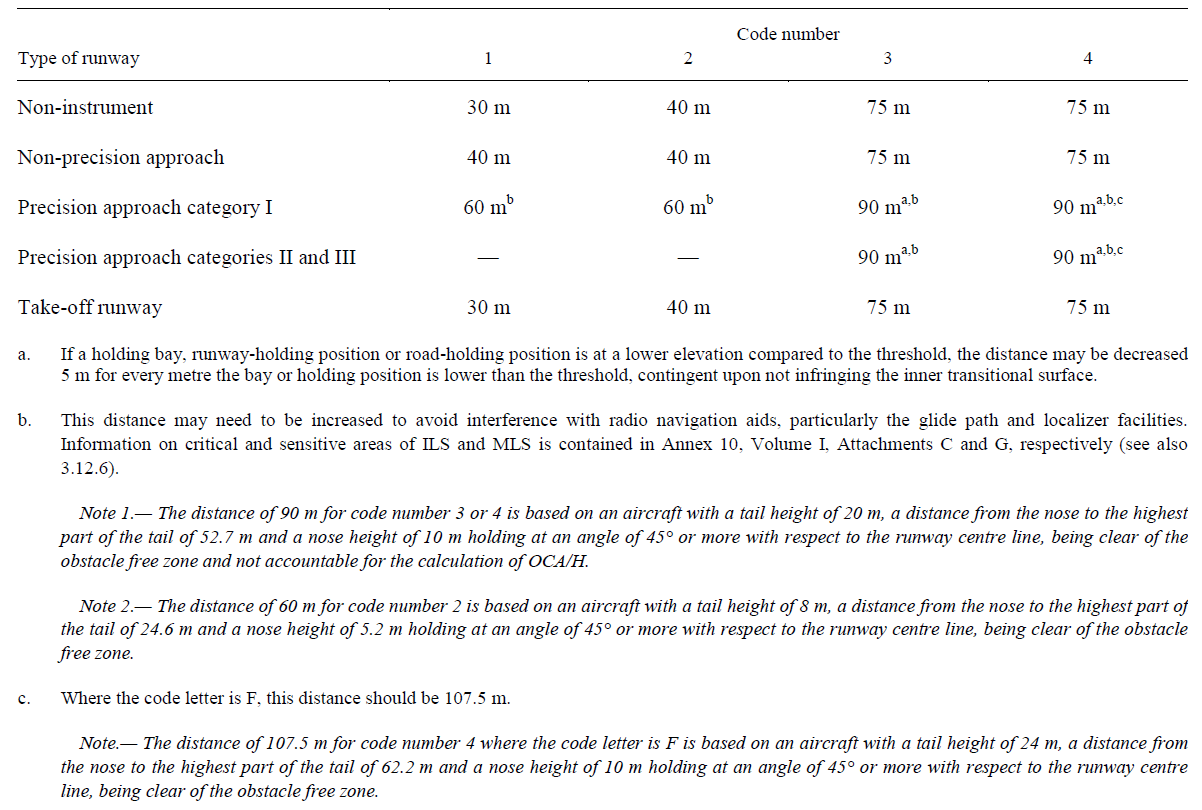
\includegraphics[clip, trim=0cm 0cm 0cm 0cm, width=1.1\textwidth]{./images/holding/distances}
		\caption{Minimum distance from the runway centre line to a holding bay, runway-holding position or road-holding position.}
		\label{distances}
	\end{figure}

	\paragraph{} Following figure \ref{distances}, minimum distances will be chosen. The location of a runway-holding position established will be such that a holding aircraft or vehicle will not infringe the obstacle free zone, approach surface, take-off climb surface or ILS/MLS critical/ sensitive area or interfere with the operation of radio navigation aids.
	
	\section{Clearance distances on aircraft stands}
	\paragraph{} An aircraft stand will provide the following minimum clearances between an aircraft entering or exiting the stand and any adjacent building, aircraft on another stand and other objects:
	
	\begin{figure}[H]
		\centering
		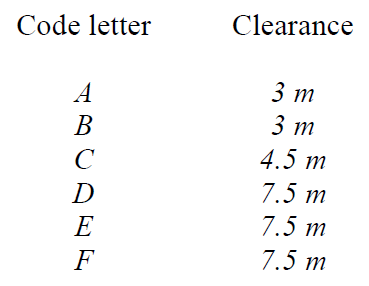
\includegraphics[clip, trim=0cm 0cm 0cm 0cm, width=0.3\textwidth]{./images/holding/clearances}
		\caption{Clearance distances on aircraft stands}
		\label{clearances}
	\end{figure}
	
	\section{Interference with critical and ILS sensible areas}
	\paragraph{} Obstacle limitation surfaces have been defined on section \textit{11. Aeronautical limitation surfaces}. Arrangements will be made to enable the appropriate authority to be consulted concerning proposed construction beyond the limits of the obstacle limitation surfaces that extend above a height established by that authority, in order to permit an aeronautical study of the effect of such construction on the operation of aeroplanes.
	
	According to the Annex 14, section 4.3, \cite{Standards2016},in this new airport, there are no obstacles interceding the ILS critical areas. From document \cite{Telecomunicaciones}, figures C-4 and AC-4B, describe how planes moving over the surface can interfere with ILS area, is not the case for the airport. It can be also corroborated in the CAD model of the whole airport. 
	
	
	
	
	\section{Interference with CWY and physical obstacles}
	
	\subsection{Separation between aircraft }
	
	\section{Final design of holding positions}